%% BioMed_Central_Tex_Template_v1.06
%%                                      %
%  bmc_article.tex            ver: 1.06 %
%                                       %

%%% loading packages, author definitions

%\documentclass[doublespacing,linenumbers]{bmcart}% uncomment this for drafts and comment for final papers
\documentclass{bmcart}% uncomment this for final papers and comment for drafts

%%% Load packages
\usepackage[T1]{fontenc}
\usepackage[latin9]{inputenc}
\usepackage{graphicx}
\usepackage{verbatim}
\usepackage{amsthm,amsmath}
\usepackage{float}
\usepackage{subcaption}

%%% Begin ...
\begin{document}

%%% Start of article front matter
\begin{frontmatter}

\begin{fmbox}
\dochead{Capstone Research}


\title{Effects of Stochastic Opening Times of Caveolae on the Sinoatrial Node's Action Potential}

%%%%%%%%%%%%%%%%
%% Enter the authors here %%
%%%%%%%%%%%%%%%%

\author[
   addressref={aff1},
   corref={aff1},
   noteref={n1},
   email={rich1638@pacificu.edu}
]{\inits{JR}\fnm{Jacob} \snm{Richards}}

%%%%%%%%%%%%%%%%%%%%%%
%% Enter the authors' addresses here  %%
%%%%%%%%%%%%%%%%%%%%%%

\address[id=aff1]{                           % unique id
  \orgname{Pacific University}, 			  % university, etc
  \street{2043 College Way},                     			  
  \city{Forest Grove, OR},                        % city
  \cny{USA}                                % country
    \postcode{97116}                                % post or zip code
}

%%%%%%%%%%%%%%%%
%% Enter short notes here %%
%%%%%%%%%%%%%%%%

\begin{artnotes}
%\note{Sample of title note}     % note to the article
\note[id=n1]{Corresponding Author} % note, connected to author
\end{artnotes}
\end{fmbox}% comment this for two column layout

%%%%%%%%%%%%%%%%%
%% The Abstract begins here %%
%%%%%%%%%%%%%%%%%

\begin{abstractbox}

\begin{abstract}
    
We developed a mathematical model of the cardiac action potential in the sinoatrial node cells which include the effect of caveolae with stochastic opening times. The effects of the caveolae can be model through probability density functions. These probability density functions allow us to model the randomness of the opening and closing of the thousands of caveolae formed around the cell. Lastly, these results are compared with those of a previous mathematical model of stochastic caveolae opening development in a cardiomyocytes cell.

 \end{abstract}

%%%%%%%%%%%%%%%%%
%% The keywords begin here%%
%%%%%%%%%%%%%%%%%

\begin{keyword}
\kwd{Action Potential}
\kwd{Nernst Equation}
\kwd{Probability Distributions}
\kwd{Cardiac Cells}
\end{keyword}

\end{abstractbox}

\end{frontmatter}

%%%%%%%%%%%%
%% The Main Body %%
%%%%%%%%%%%%


\section*{Background}

\subsection*{Introduction}

Cardiac electrophysiology is the study of the electrical activity inside of your heart. The advancement of knowledge in cardiac electrophysiology allows physicians to be more informed and to make more accurate diagnosis when treating patients with certain heart conditions. Through the mathematical modeling of cardiac electrophysiology we can gain valuable insight to how the heart works along with factors that effect how the heart beats.

Cardiac cells are called excitable cells because they undergo an action potential as the cell is stimulated. The action potential of a cardiac cell is a process where the cell undergoes a large periodic change in potential across the membrane over time, due to a initial stimulus.

Once stimulated the cardiac cell will then go through a contraction phase if stimulated above a certain critical value. This process is known as excitation contraction coupling, which is the physiological process of converting an electrical stimulus to a mechanical response\cite{Besse2007} and will occur across all of the connected heart cells. This causes a group contraction of all the cardiac muscle cells in the heart. 

Many different types of mathematical models have been created in order to simulate the effects of certain factors on the cell's action potential. In particular this paper uses the model from Yanaghara, Noma, and Irisawa from their reconstruction of the sino-atrial node pacemaker potential. See the Model section of the background portion for more information about the model being used.   


\subsection*{Cell membrane as a circuit}

 The cell membrane of a cardiac cell acts as a separation between the interior and exterior cellular environment. The membrane is embedded with a variety of transport proteins, specifically ion channels which allow the transport of certain ions across the cell membrane.

%\subsection*{Cell Membrane}

\begin{figure}[h!]
  \centering
  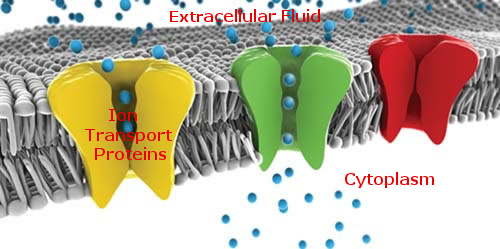
\includegraphics[width=3in]{CellMembrane.png}
  \caption[Cell Membrane]
   {The cell membrane which separates the extracellular fluid from the\\
   cytoplasm. The transport proteins act as the gateway for various ions\\
   across the membrane. \cite{CellMemPhoto} }
\label{fig:Membrane}
\end{figure}

 Figure \ref{fig:Membrane} shows the cell membrane, along with the ion transport channels. The fluctuation of ions across the membrane via these ion channels create a change in potential across the membrane. Once the change in potential hits this critical value then the membrane potential embarks on an excursion called the cardiac action potential.\cite{Besse2007}
 
 \begin{figure}[h!]
  \centering
  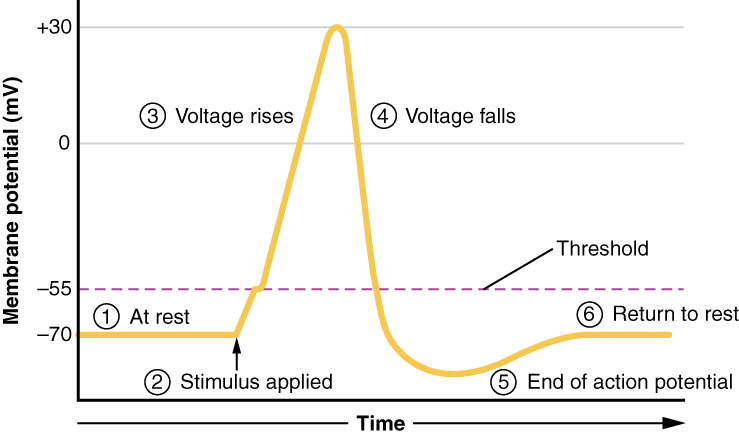
\includegraphics[width=3in]{action_potential}
  \caption[action_potential]
  {The graph of a cell going through the process of a action potential,\\
  after said stimulus. \cite{ActPotImage}}
\label{fig:actionPotential}
\end{figure}
 
 The ion species which have the greatest impact on the cell action potential are \begin{math} Ca^{+2}, \: Na^ {-1}, \: \textrm{and} \: K^{+1} \end{math}.
 
 As illustrated in figure \ref{fig:CellCircuit} a cardiac cell behaves like an electrical circuit.
 \begin{figure}[h!]
  \centering
  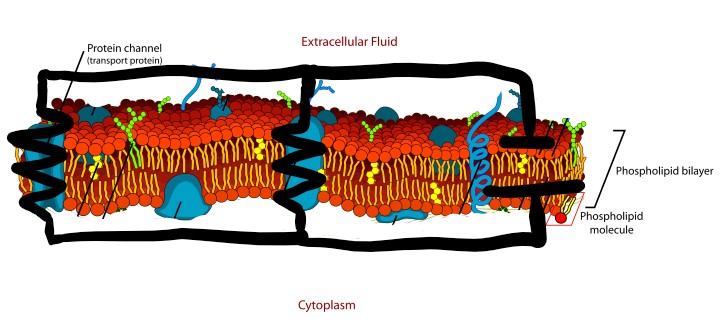
\includegraphics[width=3in]{CellCircuit}
  \caption[cell circuit]
  {The movement of ions through the ion channels create an electrical\\
  circuit which can be similar model as the above diagram. With the ion\\
  channels acting as variable resistors and the membrane as a capacitor.\cite{ElecticMem}}
\label{fig:CellCircuit}
\end{figure}

We see the ion channels act as variable resistors in the circuit along with the membrane serving as a capacitor separating the charge on the outside of the cell and the inside of the cell.
 
 \subsection*{Forces on Ions}
 
 There are two main forces which dictate the movement of ions: diffusion, and electrophoresis. Diffusion is the chemical force which acts upon molecules moving them in a direction from high concentration to low  concentration. Electrophoresis is the electrical force on the ion that comes from the force applied from an electric field.\cite{Besse2007}

\subsection*{Force on the Ions}

 \begin{figure}[h!]
  \centering
  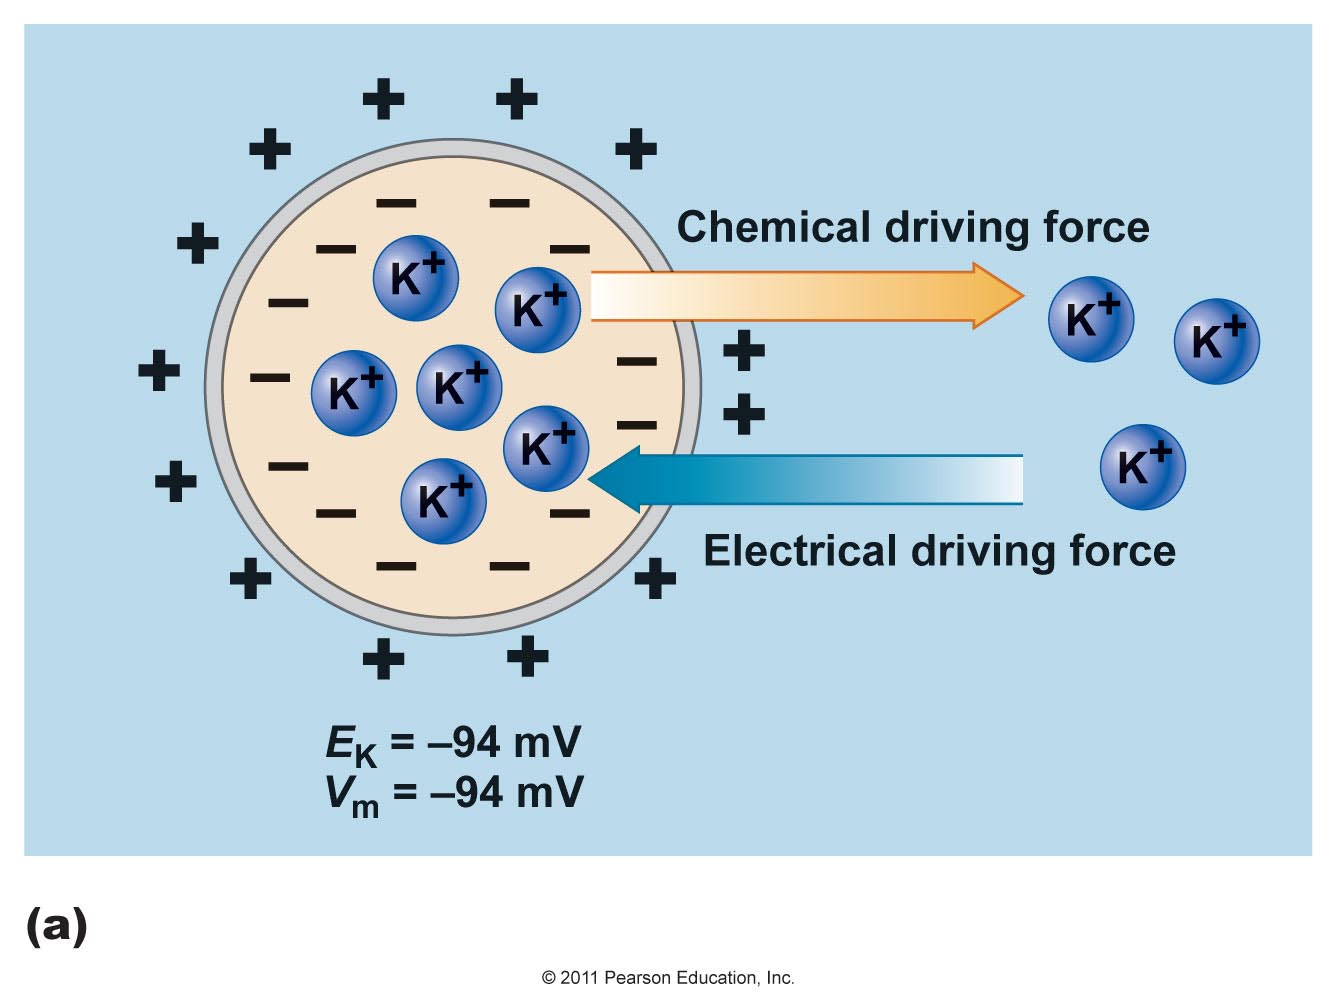
\includegraphics[width=3in]{forcesOnIons}
  \caption[cell circuit]
  {The two forces which act on a ion will be a chemical and electrical\\
  force. The chemical forces pushes the ion in the direction of high \\
  concentration to low concentration, while the electrical force moves\\
  ions of like charges together and ions of opposing charges away from \\
  each other. \cite{ForcesOnIons}}
\label{fig:IonForces}
\end{figure}

Figure \ref{fig:IonForces} shows that two forces which act on the ions, both a chemical and electrical force.

\begin{equation}
\\
$$
 J_T = -\mu_S \left( \frac{RT}{F} \cdot \frac{\partial [S]}{\partial x} + z_S [S] \frac{\partial v}{\partial x} \right)
$$
 \label{NernstFluxEquation}
\end{equation}

This Equation (\ref{NernstFluxEquation}) is made up of both forces acting on a specific ion species in a cardiac cell, and gives the total molar flux, also known as the Nernst-Planck molar flux equation.

\subsection*{Nernst Equation}

The Nernst Potential, for a specific ion is the membrane potential that results in zero net flux. 

 \begin{figure}[h!]
  \centering
  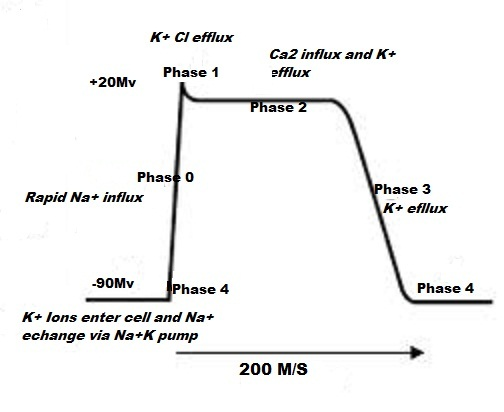
\includegraphics[width=2in]{ActionPotential}                                                              
  \caption[Action Potential]
  {Action Potential of a cardiac cell. \cite{ActionPoten2}}
\label{fig:ActionPotential}
\end{figure}

\begin{equation}
\\
$$
 E_S = \left (\frac{R T}{z_S F} l n \frac {[S]_0}{[S]_i} \right)
$$
\label{NernstEquation}
\end{equation}

Equation (\ref{NernstEquation}) shows \begin{math} E_S \end{math} being the Nernst potential for a specific ion S. Which represents the potential that a species of ion tries to reach in order to obtain equillibrium\cite{Besse2011}.

 Earlier we mentioned the cell membrane shows similar properties to that of an electrical circuit. Because of this we can use Kirkoff's law when modeling a cell's action potential. Kirkoff law states that the currents within a system must sum to zero. The currents which are active in our model our the ionic currents and the current from the membrane. the membrane has a current since it acts like a capacitor. By manipulating the set of currents inside of the cell using kirkoff's law we can come to the conclusion below.
\begin{equation}
\\
$$
I_{Na} \: + \: I_{Ca} \: + \: I_K \: + \: I_{C_m} \: = \: 0
$$
\label{ModelBase}
\end{equation}
\begin{equation}
          \\
   $$
 I_{C_m}  = C_m \: \cdot \: \frac {d V_m}{d t} 
    $$          
    \end{equation}
    Change of Voltage Across Membrane Over Time:
    \begin{equation}
      \\
    $$
  \frac {d V_m}{d t} \color{black} = - \frac {1}{C_m}(I_{Na} \: + \: I_{Ca} \: + \: I_K \:)
$$
\label{ModelBaseFour}
    \end{equation}
    
Equation \ref{ModelBaseFour} can be simplified such that we can write it as,
\begin{equation}
\\
$$
 (\frac {d V_m}{d t}) = - \frac {1}{C_m}(\sum \nolimits_{S \in \Omega} I_S ) 
$$
\\
$$
 \Omega = (Na, k, Ca)
$$
\label{ModelTwo}
\end{equation}

Equation (\ref{ModelTwo}) is the base for modeling the action potential of a cell. Hodgkin and Huxley, two prominent leaders in the field, took this idea and characterized each current based off of the ion channels associated with the current. Look in Equations and Models sections to see more detail.

\section*{Equations and Models}

\subsection*{Hodgkin and Huxley Model}

Hodgkin and Huxley were able to come up with models for the Na and K currents known as the Hodgkin-Huxley formalism,\cite{Sneyd2016}. The process for their formalism starts from the following ion current equation below. Equation (\ref{ModelThree})
\begin{equation}
\\
$$
    I_S = g_S (V_m - E_s)
$$
\label{ModelThree}
\end{equation}

Where \begin{math} V_m - E_s \end {math} of the model for a ion species current is the part of the model which acts as the driving force on the ions. $E_s$ value is the Nernst potential which each ion species tries to get membrane potential, $V_m$, in order to reach a stat of no net flux. This leaves us with \begin{math} g_S \end{math} which is the resistance of a said ion species. Hodgkin and Huxley then express \begin{math} g_S \end{math} as the product of the maximum possible ion species current and a set of gating variables defined by their own differential,\cite{Sneyd2016}.\\
For example the Hodgkin-Huxley formalism for \begin{math}  Na \end{math} is,
\begin{equation}
\\
$$
    I_{Na} = \overline{g_{Na}} m^3 h (V_m - E_{Na})
$$
\label{NaForm}
\end{equation}

to continue these gates, $m$ and $h$, obey a set of differentials,
\begin{equation}
\\
$$
    \frac {d m}{d t} =  \frac {m_{\infty} (V_m) - m}{\tau_m (V_m)}
$$
\label{changeM}
\end{equation}
\begin{equation}
\\
$$
   \frac {d h}{d t} =  \frac {h_{\infty} (V_m) - h}{\tau_h (V_m)}  
$$
\label{changeH}
\end{equation}

 When we take into consideration Hodgkin-Huxley formalism our base model now takes the following form, 
\begin{equation}
\\
$$
\frac {d V_m}{d t} = - \frac {1}{C_m} (\overline{g_{Na}} m^3 h (V_m - E_{Na}) + \overline{g_K} n^4 (V_m - E_{K}) +  \overline{g_{CA}} df (V_m - E_{Ca}))
$$
\label{ModelBaseFinal}
\end{equation}

This only acts as a base model for a very rudimentary situation. In order to create a more accurate model we will need to incorporate a larger variety of ionic currents from within the cell.
\\

\subsection*{Yanagihara, Noma, and Iri-saw model}

The parent model we will be using specifically for our project is from Yanagihara, Noma, and Irisawa in their paper on the reconstruction of sino-atrial node pacemaker potential. Their model consisted of modeling six specific currents; \begin{math} i_s,\: i_{Na},\: i_h,\: i_k,\: i_1,\: and \: i_m \end{math}\cite{Yanaghara1980}. 

\begin{equation}
\\
$$
\frac {d V_m}{d t} = - \frac {1}{C_m}(I_h \: + \: I_l \: + \: I_{Na} \: + \: I_{Ca} \: + \: I_K \:)
$$
\label{YangBase}
\end{equation}  


Each current will expand as follows:
\\
$i_s = (.95d)+.05)\cdot(.95f+.05)\cdot (12.5 \cdot (e^{(V - 10)/15} - 1)) $

The gating mechanism for calcium is governed by two gating variables $d$ and $f$
\\
$i_{Na} = m^3\cdot h \cdot (.5 \cdot (V - 30))$

The gating mechanism for Sodium is governed by two gating variables $m$ and $h$
\\
$i_h = q \cdot (.4 \cdot (V + 45))$

The gating mechanism for the Hyper-polarization-activated current is governed by one gating variables $q$
\\
$i_k = ((.7 \cdot p) \cdot (e^{.0277\cdot(V+90)}-1))/e^{.0277 \cdot (V + 40)})$

Potassium Current channel consist of one gated type variables $p$ also referred to as $n$ in other models
\\
$i_1 = .8(1-e^{-(E+60)/20)})$

Leak Current channel consist of no gated type variables since the current comes from the gap junctions in the membrane.  
\\
\cite{CellML}
The currents above are chosen to model a SA node of a rabbit. They may change as the caveolae factors are added to the model, since caveolae could hold a variety of ion channels. When they are open The cell is able to access the ion channels in the caveolae, which can result in a change in the action potential. 


\section*{Effects of Cardiac Caveolae}
\subsection*{Caveolae}

\begin{figure}[h!]
  \centering
  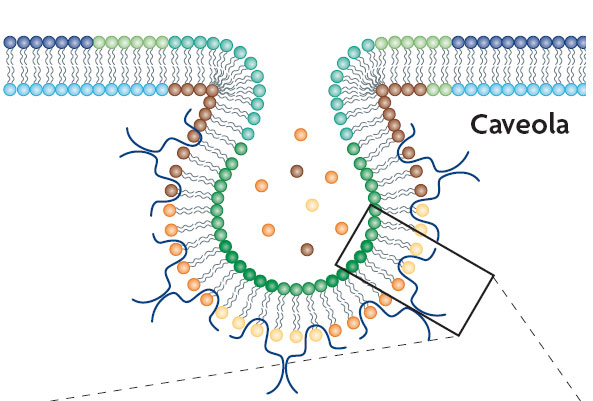
\includegraphics[width=3in]{cavealoa}
  \caption[cavealoa]
  {A single caveolae in the cell membrane}
\label{fig:ActionPotential2}
\end{figure}

Our model takes into consideration the effects of the caveolae on the SA node. The ion currents from the caveolae will be characterized differently from their sibling currents around the cell membrane, based on the fact that research shows caveolae can be either open or closed.

\section*{Our Model}
The caveolae are held closed by a specific structural protein. Only through a specific pathway do these proteins retrieve the signal which allows them to shift in their structure and for the caveolae to open up. In order to incorporate this into our model we will be using an exponential distribution in order to obtain the waiting time for each caveolae that open up during the action potential of a given SA Node\cite{Barb06} . 

It is unsure what the Mu factor would be for a given exponential distribution, so for our experiments we will be using mu factors of 2ms, 10ms, 100ms,and 1000ms in order to see which results would best match the opening behavior of caveolae in the SA Node. We also incorporated a mechanism into our code which allows our caveolae to stay opened for a set time of 5ms. While the caveolae is open it will be releasing a current based on the sum of the current of the ion channel type present.

A key factor of our model is the ability for our caveolae to open and also close. Previous models looked are base one a caveolae just opening once during the cycle of an cell's action potential. Our model will be taking into consideration that a caveolae will open and close multiple times throughout the process of a cell's action potential. 

In order to incorporate this action of our caveolae opening and closing into our model we created a 30,000 by 700 matrix. Each column in our matrix contains a the individual opening of the caveolae during the action potential process. Our matrix became a sequence of wait times which we derived from the exponential distribution. The exponential distribution has a mu value associated with it which is the average random value for the exponential distribution. In our model we can think of it as our average waiting time a caveolae has to wait to open based on an exponential distribution. We made sure to check the opening times of the caveolae in our last row of our matrix just in case when we generated our matrix it didn't get filled all the way, since their is a small probability that a caveolae could have a large set of short opening times\cite{Zhu2015}.

Previous models looked at also did not look at the sinoatrial node. Our model looks specifically at the sinoatrial node, which posses a different type of action potential then most cardiac cells based on the fact that it has the ability to spontaneously produce an electrical impulse.

Based on previous research, we know as the caveolae open the sodium channels inside the caveolae will have a effect on the cells action potential\cite{Besse2007}. But recently, research has shown caveolae hold a variety of ion channels, which is why we will be experimenting with what effects different types of ion channels have when they are present in the caveolae.

Our model will look into the specific effects that the \begin{math} Ca^{+2}, \: Na^ {-1}, \: \textrm{and} \: K^{+1} \end{math} ion channels individually have inside the caveolae on SA node. 

The currents within a caveolae follow an ion current equation that differs slightly from the ion current equation for our entire model, since it will be based on a single ion channel conductance rather then a cell ion channel conductance. Because of this the current from an ion channel inside a caveolae will follow the equations below\cite{Ronald2007}.

If the ion channel is opened:
\begin{equation}
\\
  $$
   I_S = \gamma_S \color{black} (V_m - E_s)
  $$
\label{CavCurrentEqu}
\end{equation}

\begin{math} \gamma_S \end{math} is the single channel conductance of a single ion channel.

Each ion channel will produce the current for it's specific type, if it in open or closed. In order to incorporate if the ion channel was open or closed in our model we developed a mechanism in our code which told us if the ion channel was open or closed based on the gating variables of that specific ion channel. 

We created a random matrix for each ion channel 30,000 by "n" where "n" is the number of gates the ion channel possess. Each one of these gates were a 1x30,000 matrix which contained a value of 1 or 0. If they value was 0 then the gate would be closed, and then the whole ion channel would be closed. The only way a ion channel could be open was if all the gates were 1 in its respected column of the ion channel matrix.

This 1 and 0 value were computed by developing a method such that the matrix index of that gated variable would be equated to the steady state value of the gating variable based on a fixed membrane potential. So each ion channel has a probability of being open based on it's own ionic species. What our mechanism does is allows for our ion channels within our model to hold to these properties. 
    
Based on the additions of the sum of the caveolar currents during a set time within the cell membrane we come to the conclusion of the model below. 
\begin{equation}
\\
 $$
\frac {d V_m}{d t} = - \frac {1}{C_m}(I_h \: + \: I_l \: + \:I_{Na} \: + \: I_K \: + \: I_{Ca} \: + $$ $$ \sum \nolimits_{Cav \in \Omega} I_{Cav})
$$
\label{OurModel}
\end{equation}
\\
$$
 \Omega = (Cav_{Na}, Cav_k, Cav_{Ca}, Cav_l, Cav_h)
$$

\section*{Results}

For our experiments we ran our model in MATLAB. The first set of experiments we ran were with each caveolae containing a single calcium ion channel. We then experimented with the mu factor we spoke of earlier to see the effects. The blue line represents a SA nodes action potential without the effects of caveolae.
As we can see the calcium will prolong the peak of the action potential, while also causing early depolarization at certain moments in time.

The next set of experiments we ran involved the same process but with sodium. With sodium we noticed the surplus of sodium prolong the peak of the action potential, while increasing the frequency of the action potential cycle. 

We then ran the same tests with potassium. The surplus of potassium will cause a shift towards a more negative action potential given its strong negative nernst potential, which logically make sense. 

Lastly we decided to test the hyper polarization current and noticed it will prolong the peak while also raising the peak of the action potential constantly over time. It will even cause early depolarization randomly at some points in the process. When it comes to our mu factor we notice the mu factor is more likely to be larger since it more realistically follows that of a SA node action potential. Which means the caveolae are more likely to open up at a slower pass during the action potential phase then opening up at a fast pace based on our models properties.

\section*{Further Research}

 Further research using this model would include experimentation with multiple ion channels inside the caveolae at once. Also further research would include additions to this model to take into consideration the surface area of caveolae when they open up since we believe they would have a effect on the capacitance of the cell membrane. 

%\section*{Details of Model}

\section*{Graphs}

\begin{figure}[ht]
  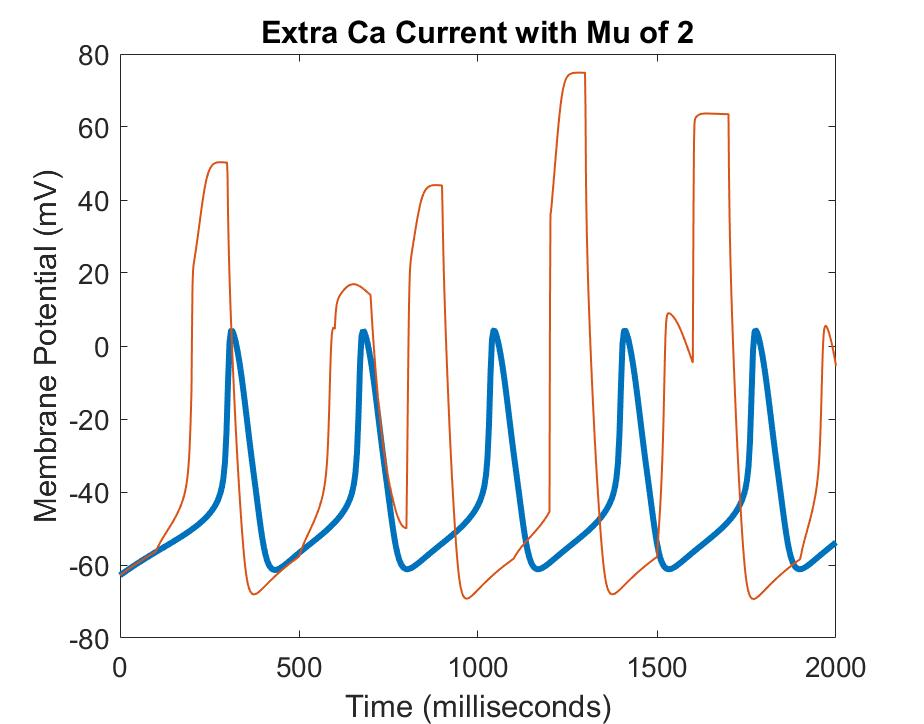
\includegraphics[width=3in]{images/CaMu2}
  \caption[CacliumMu2]
  {Experiment with caveolae containing a single calcium ion channel\\
  with a mu factor of 2}
\label{fig:CaMu2}
\end{figure}

\begin{figure}[ht]
  \centering
  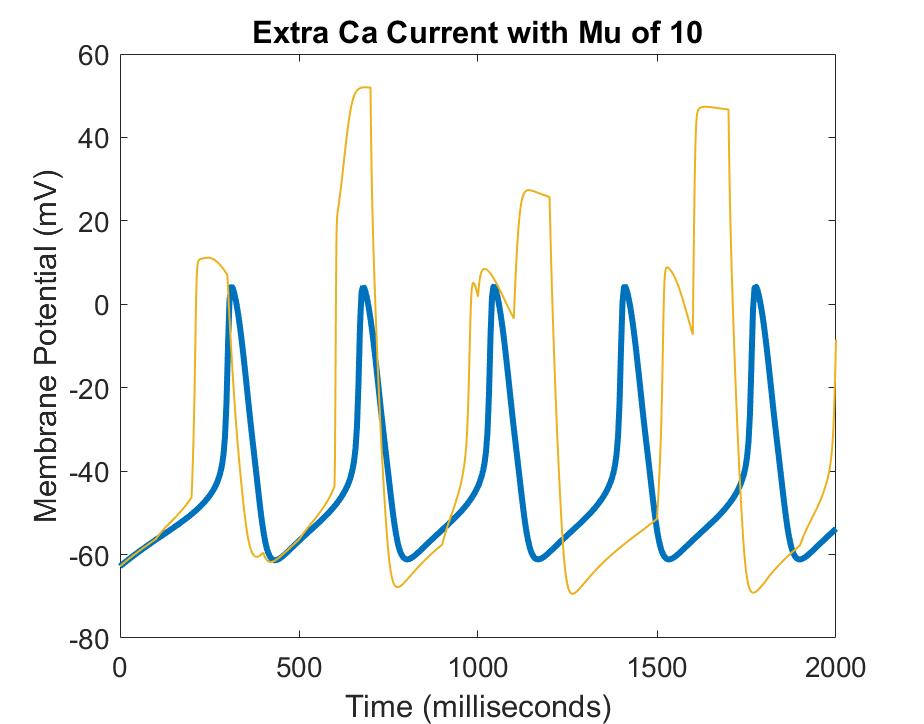
\includegraphics[width=3in]{images/CaMu10}
  \caption[CacliumMu10]
  {Experiment with caveolae containing a single calcium ion channel\\
  with a mu factor of 10}
\label{fig:CaMu10}
\end{figure}

\begin{figure}[ht]
  \centering
  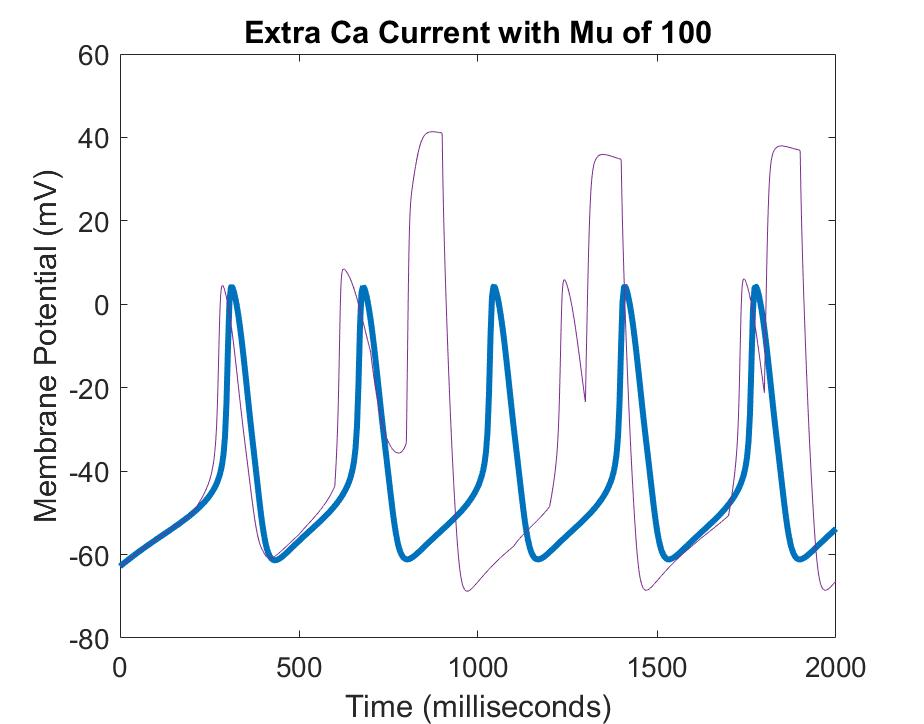
\includegraphics[width=3in]{images/CaMu100}
  \caption[CacliumMu100]
  {Experiment with caveolae containing a single calcium ion channel\\ 
  with a mu factor of 100}
\label{fig:CaMu100}
\end{figure}

\begin{figure}[ht]
  \centering
  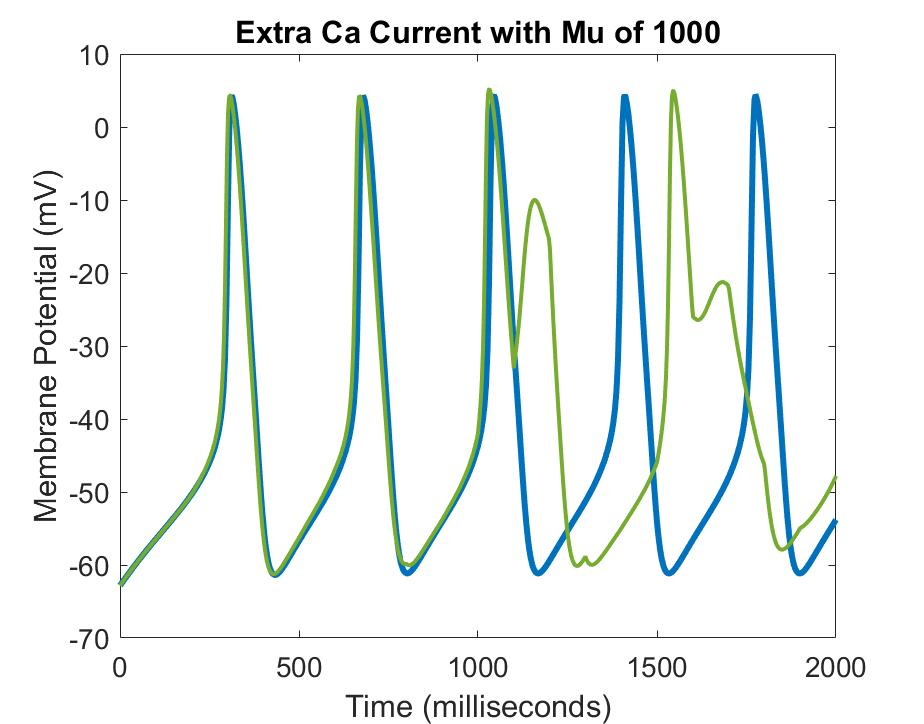
\includegraphics[width=3in]{images/CaMu1000}
  \caption[CacliumMu1000]
  {Experiment with caveolae containing a single calcium ion channel\\
  with a mu factor of 1000}
\label{fig:CaMu1000}
\end{figure}
 
%%-------------------------------------------------------------------

\begin{figure}[ht]
  \centering
  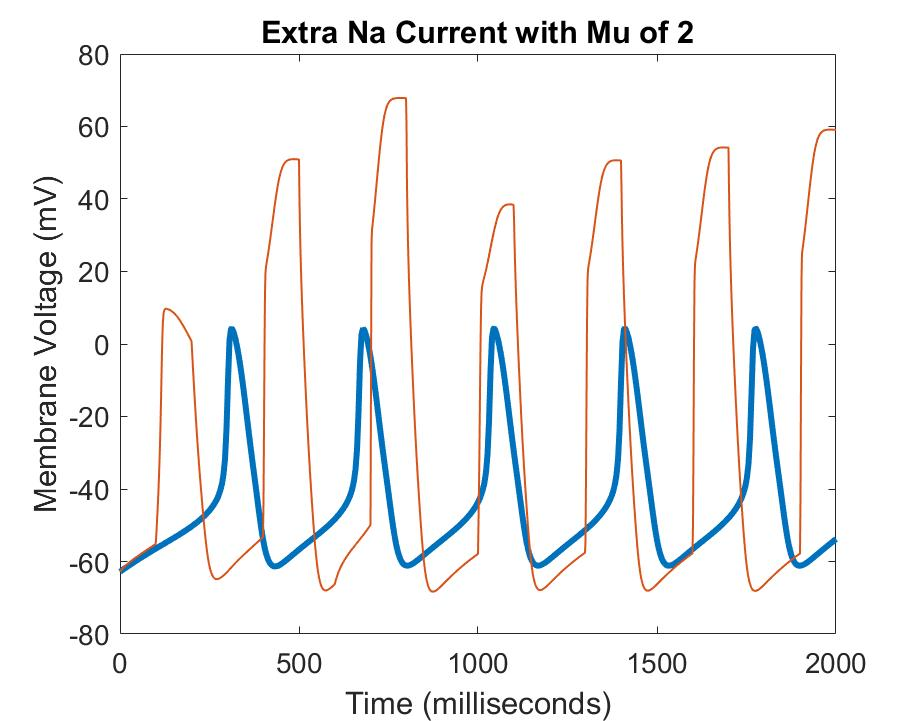
\includegraphics[width=3in]{images/NaMu2}
  \caption[SodiumMu2]
  {Experiment with caveolae containing a single sodium ion channel\\
  with a mu factor of 2}
\label{fig:NaMu2}
\end{figure}

\begin{figure}[ht]
  \centering
  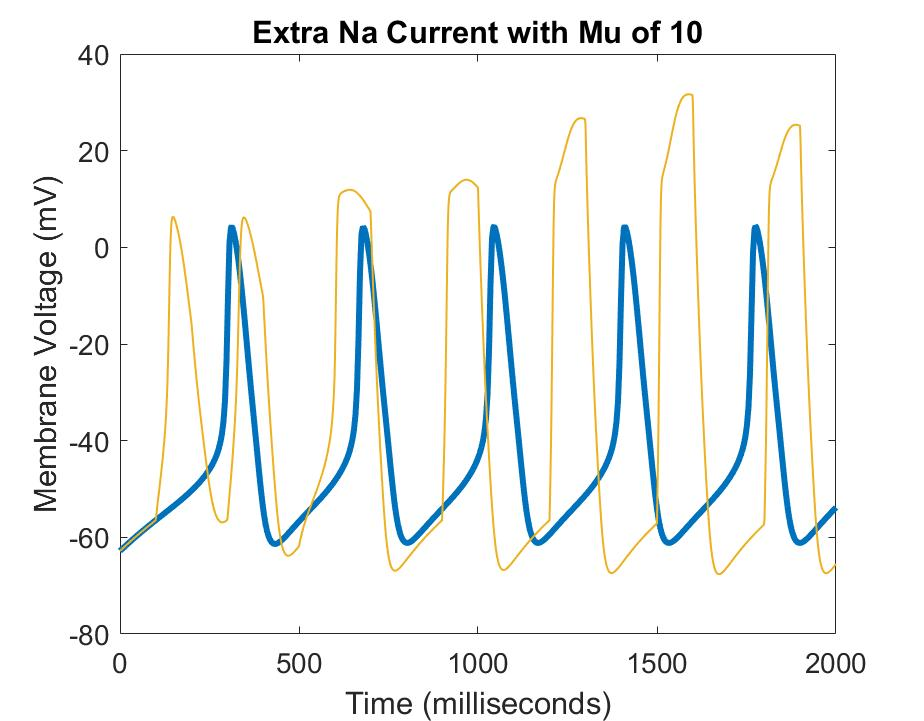
\includegraphics[width=3in]{images/NaMu10}
  \caption[SodiumMu10]
  {Experiment with caveolae containing a single sodium ion channel\\
  with a mu factor of 10}
\label{fig:NaMu10}
\end{figure}

\begin{figure}[ht]
  \centering
  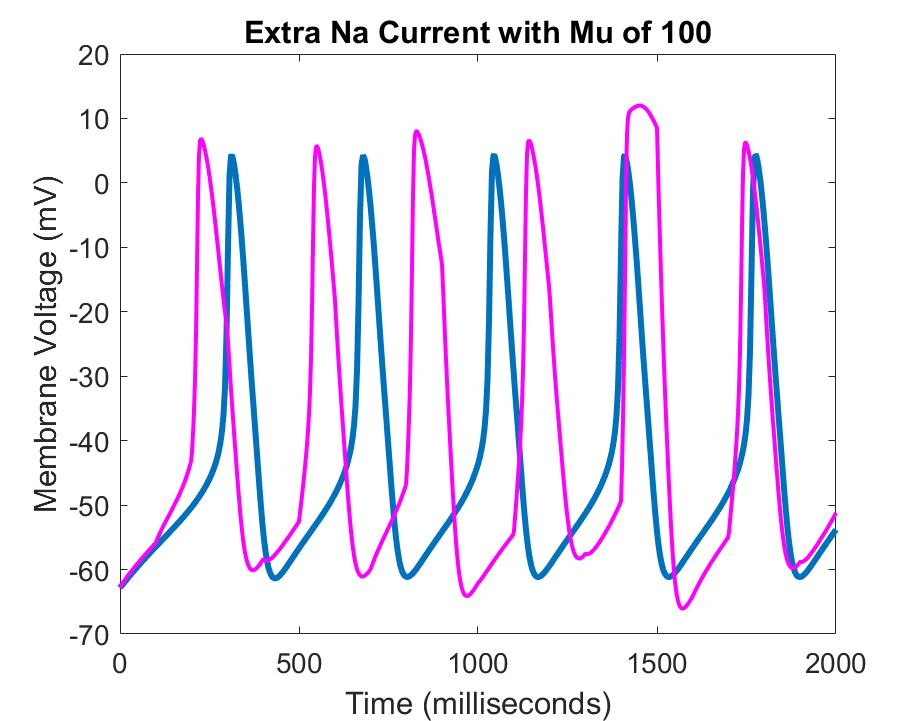
\includegraphics[width=3in]{images/NaMu100}
  \caption[SodiumMu100]
  {Experiment with caveolae containing a single sodium ion channel\\
  with a mu factor of 100}
\label{fig:NaMu100}
\end{figure}

\begin{figure}[ht]
  \centering
  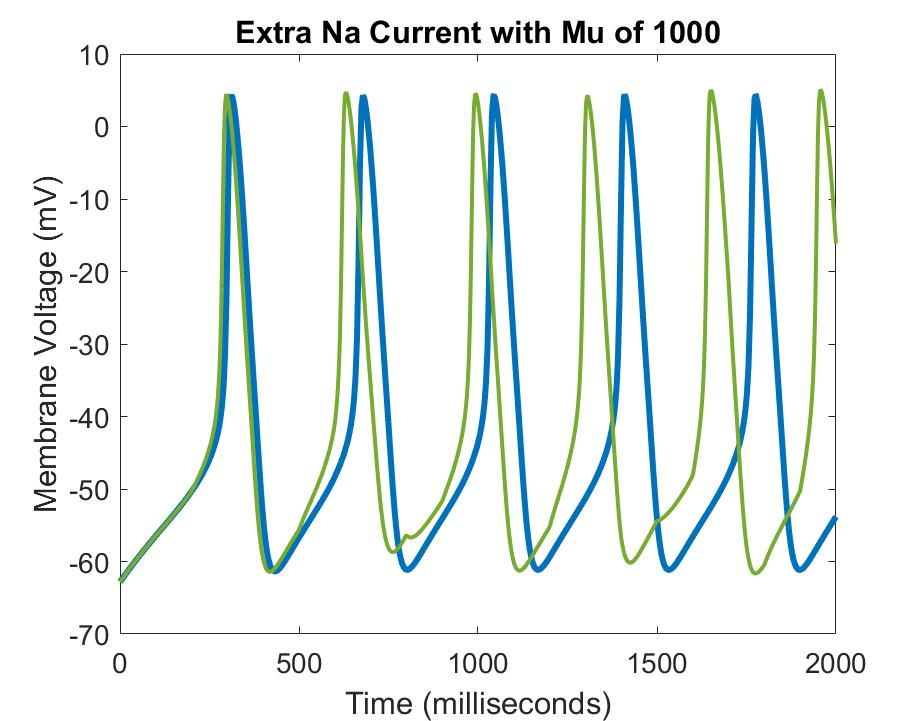
\includegraphics[width=3in]{images/NaMu1000}
  \caption[SodiumMu1000]
  {Experiment with caveolae containing a single sodium ion channel\\
  with a mu factor of 1000}
\label{fig:NaMu1000}
\end{figure}

%%-------------------------------------------------------------------

\begin{figure}[ht]
  \centering
  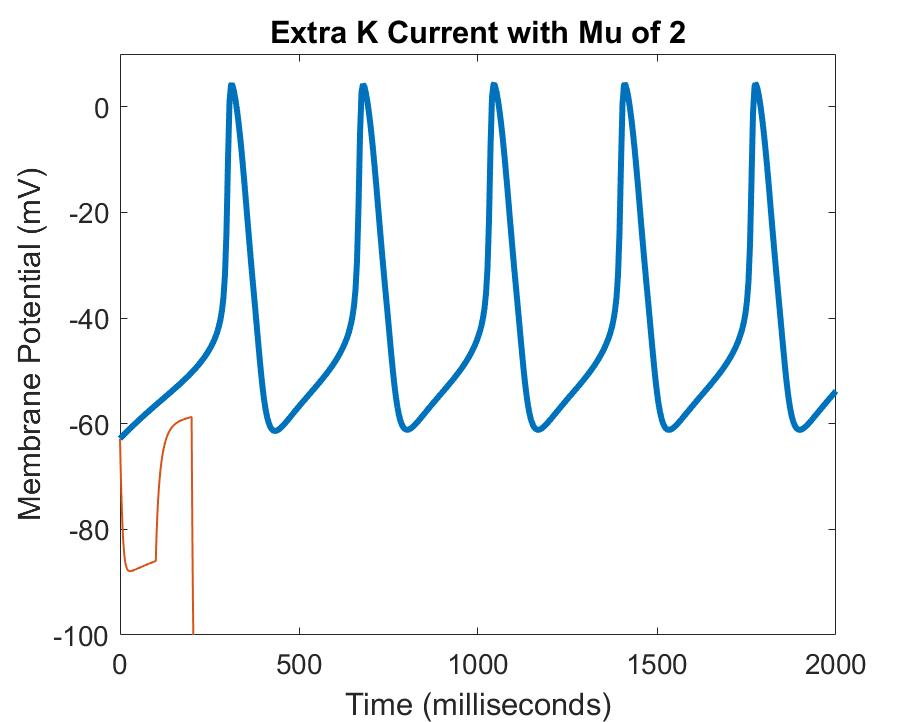
\includegraphics[width=3in]{images/KMu2}
  \caption[KMu2]
  {Experiment with caveolae containing a single potassium ion channel\\
  with a mu factor of 2}
\label{fig:KMu2}
\end{figure}

\begin{figure}[ht]
  \centering
  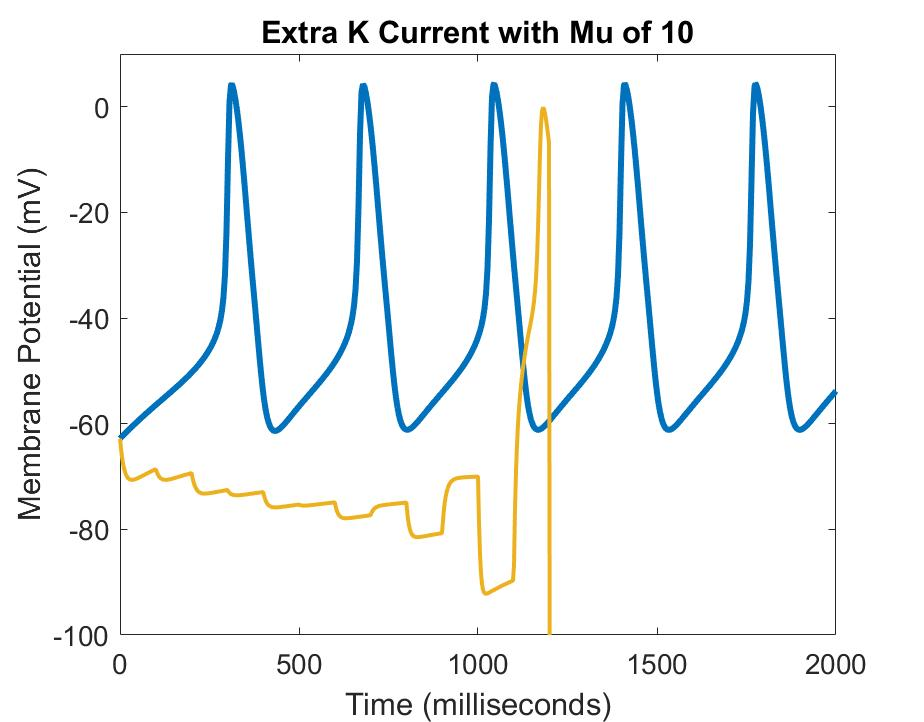
\includegraphics[width=3in]{images/KMu10}
  \caption[KMu10]
  {Experiment with caveolae containing a single potassium ion channel\\
  with a mu factor of 10}
\label{fig:KMu10}
\end{figure}

\begin{figure}[ht]
  \centering
  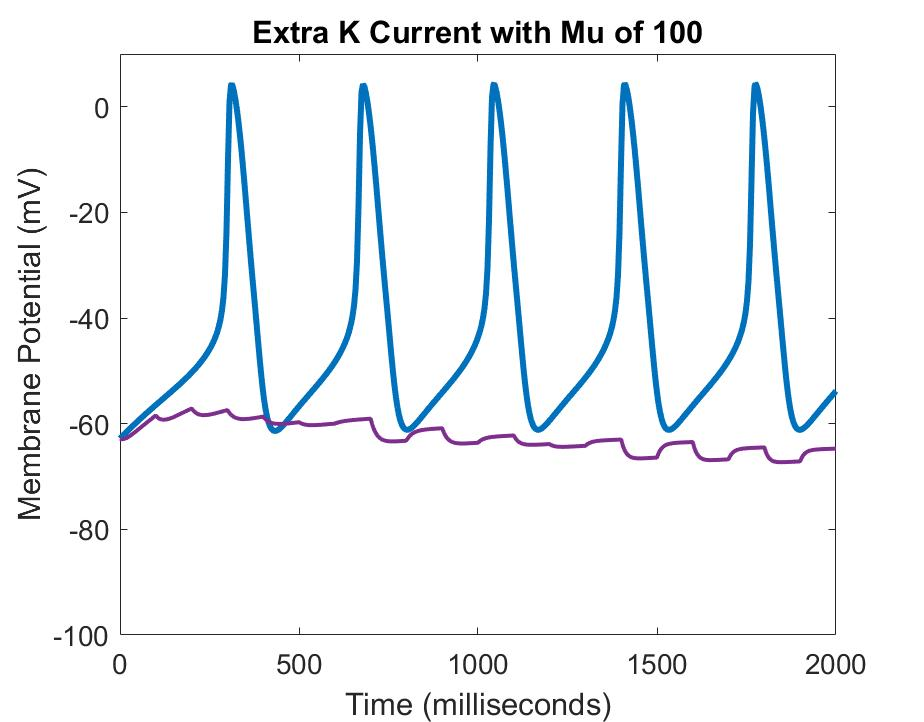
\includegraphics[width=3in]{images/KMu100}
  \caption[KMu100]
  {Experiment with caveolae containing a single potassium ion channel\\
  with a mu factor of 100}
\label{fig:KMu100}
\end{figure}

\begin{figure}[ht]
  \centering
  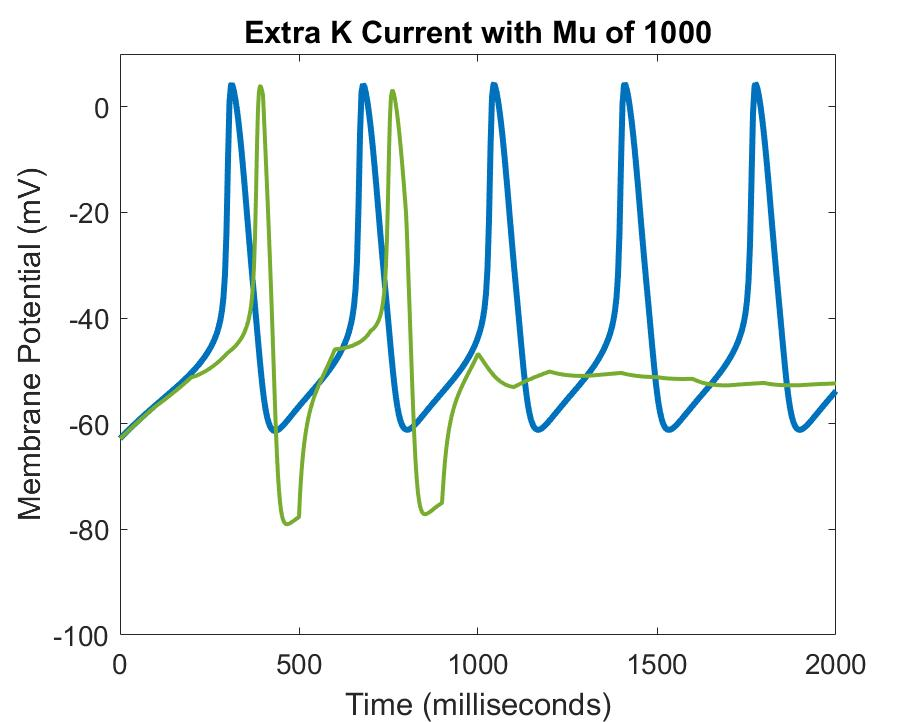
\includegraphics[width=3in]{images/KMu1000}
  \caption[KMu1000]
  {Experiment with caveolae containing a single potassium ion channel\\
  with a mu factor of 1000}
\label{fig:KMu1000}
\end{figure}

%%-------------------------------------------------------------------

\begin{figure}[ht]
  \centering
  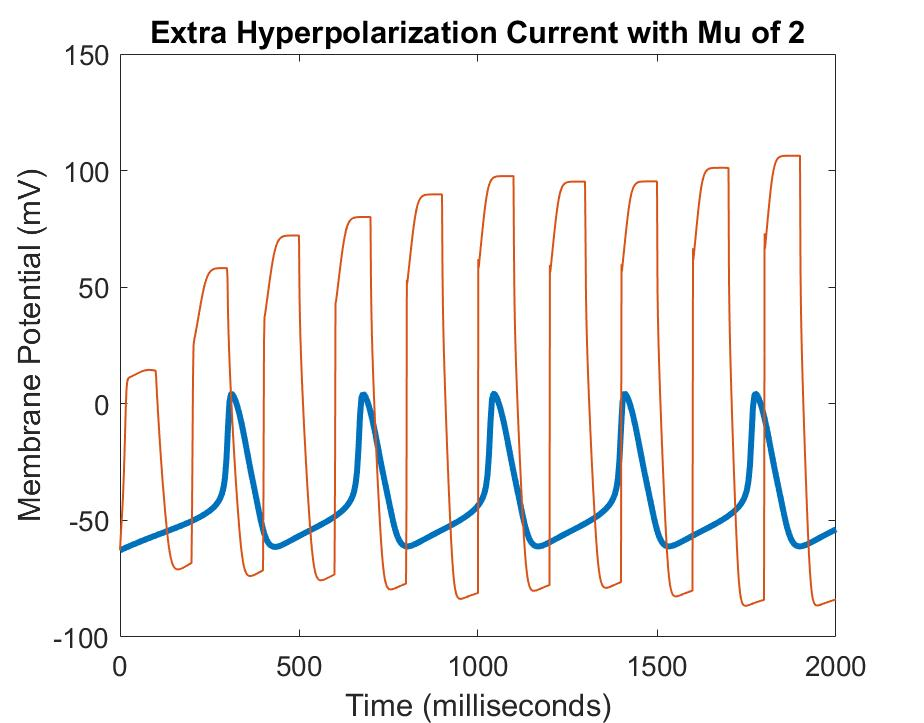
\includegraphics[width=3in]{images/hMu2}
  \caption[hMu2]
  {Experiment with caveolae containing a single hyper polarization ion\\
  channel with a mu factor of 2}
\label{fig:hMu2}
\end{figure}

\begin{figure}[ht]
  \centering
  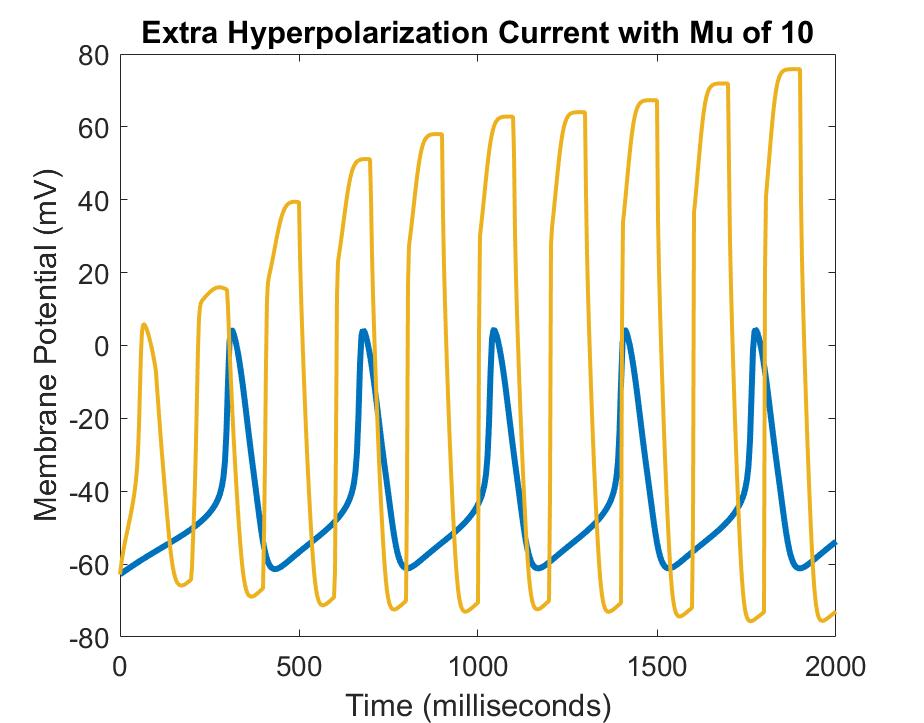
\includegraphics[width=3in]{images/hMu10}
  \caption[hMu10]
  {Experiment with caveolae containing a single hyper polarization ion\\
  channel with a mu factor of 10}
\label{fig:hMu10}
\end{figure}

\begin{figure}[ht]
  \centering
  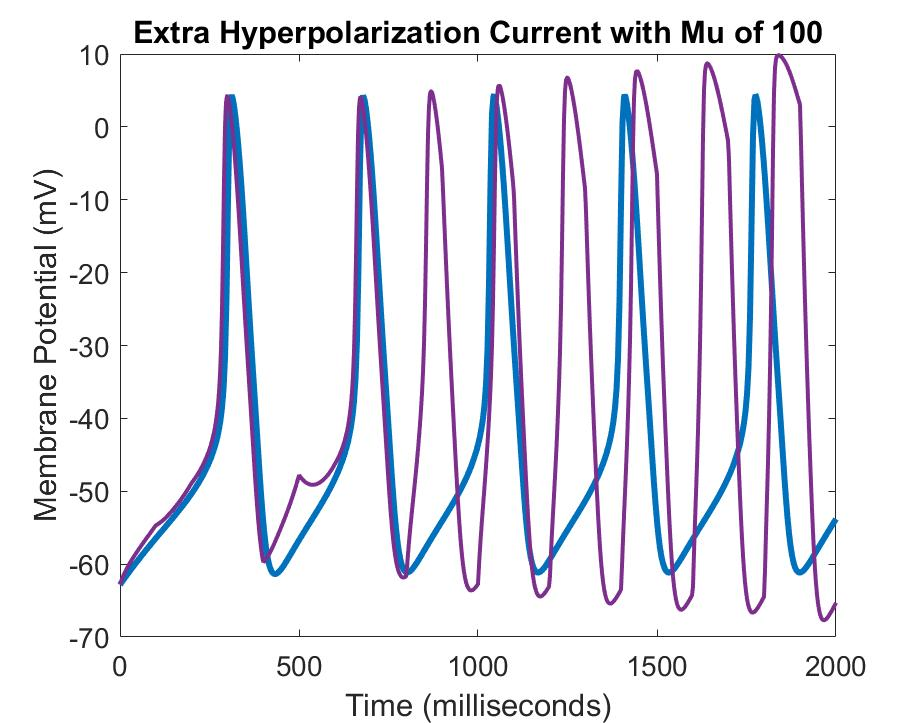
\includegraphics[width=3in]{images/hMu100}
  \caption[hMu100]
  {Experiment with caveolae containing a single hyper polarization ion\\
  channel with a mu factor of 100}
\label{fig:hMu100}
\end{figure}

\begin{figure}[ht]
  \centering
  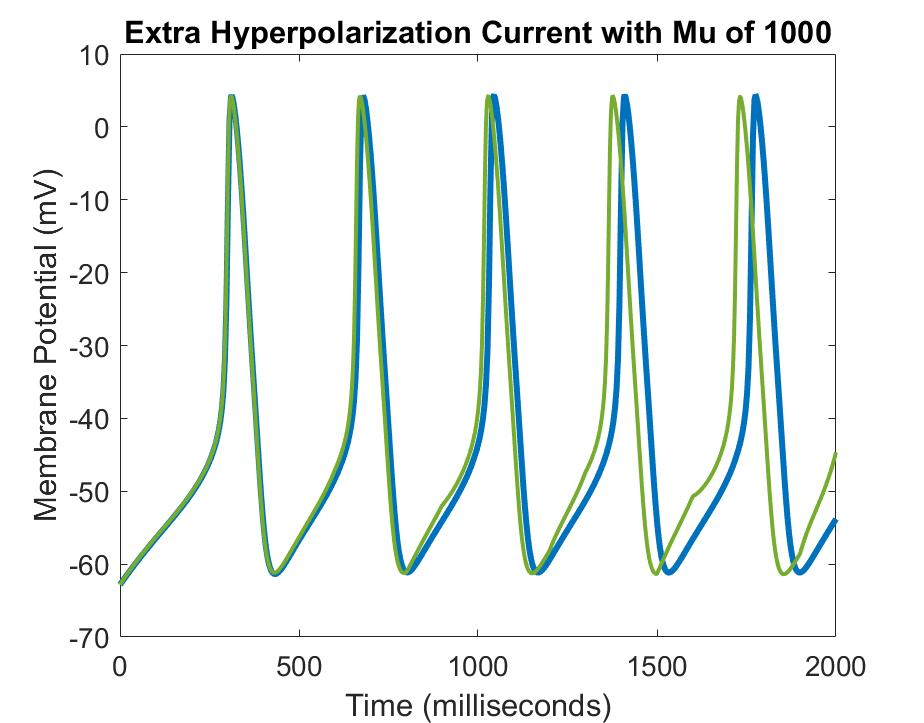
\includegraphics[width=3in]{images/hMu1000}
  \caption[hMu1000]
  {Experiment with caveolae containing a single hyper polarization ion\\
  channel with a mu factor of 1000}
\label{fig:hMu1000}
\end{figure}


\pagebreak

%%%%%Label the last page so that your pagination can reference for which page is last.
\label{LastPage}

%%%%%Now insert your bibliography. You can choose from a number of different reference styles, but the following is a good one.
\bibliographystyle{bmc-mathphys}
\bibliography{BibtexSample}

\end{document}


%%%%%%% need to cite pictures, quick grammar check, redo conclusion